\let\negmedspace\undefined
\let\negthickspace\undefined
\documentclass[journal]{IEEEtran}
\usepackage[a5paper, margin=10mm, onecolumn]{geometry}
\usepackage{tfrupee}

\setlength{\headheight}{1cm}
\setlength{\headsep}{0mm}

\usepackage{gvv-book}
\usepackage{gvv}
\usepackage{cite}
\usepackage{amsmath,amssymb,amsfonts,amsthm}
\usepackage{algorithmic}
\usepackage{graphicx}
\usepackage{textcomp}
\usepackage{xcolor}
\usepackage{txfonts}
\usepackage{listings}
\usepackage{enumitem}
\usepackage{mathtools}
\usepackage{gensymb}
\usepackage{comment}
\usepackage[breaklinks=true]{hyperref}
\usepackage{tkz-euclide} 
\usepackage{listings}

\graphicspath{{./figs/}}

\begin{document}
\title{2.6.18}
\author{AI25BTECH11010 - Dhanush Kumar}
\maketitle
\renewcommand{\thefigure}{\theenumi}
\renewcommand{\thetable}{\theenumi}

\noindent
\textbf{Question:} \\
ind the area of region bounded by the triangle whose vertices are (–1, 0), (1, 3) and
(3, 2).
\bigskip
\noindent
\textbf{Solution:}\\
 \begin{table}[H]    
      \centering
      \begin{tabular}{|c|c|}
\hline
\textbf{Name} & \textbf{Value} \\ \hline
$\vec{A}$ & $\myvec{2 & 1 \\0 & 3}$ \\ \hline
\end{tabular}

      \caption{Variables Used}
      \label{}
    \end{table}

The area of a triangle ABC is given by :

\begin{align*}
\frac{1}{2}\,\lVert \vec{(A-B)}\times\vec{(A-C)}\rVert
\end{align*}


\begin{align}
   \vec{A}-\vec{B} = \myvec{-1 \\ 0} - \myvec{1 \\ 3} = \myvec{-2 \\ -3}
\end{align}

\begin{align}
   \vec{A}-\vec{C} = \myvec{-1 \\ 0} - \myvec{3 \\ 2} = \myvec{-4 \\ -2}
\end{align}


\begin{align}
\frac{1}{2}\,\lVert \vec{(A-B)}\times\vec{(A-C)}\rVert = 4
\end{align}

\bigskip
The area of the triangle ABC is 4


\begin{figure}[h!]
  \centering
   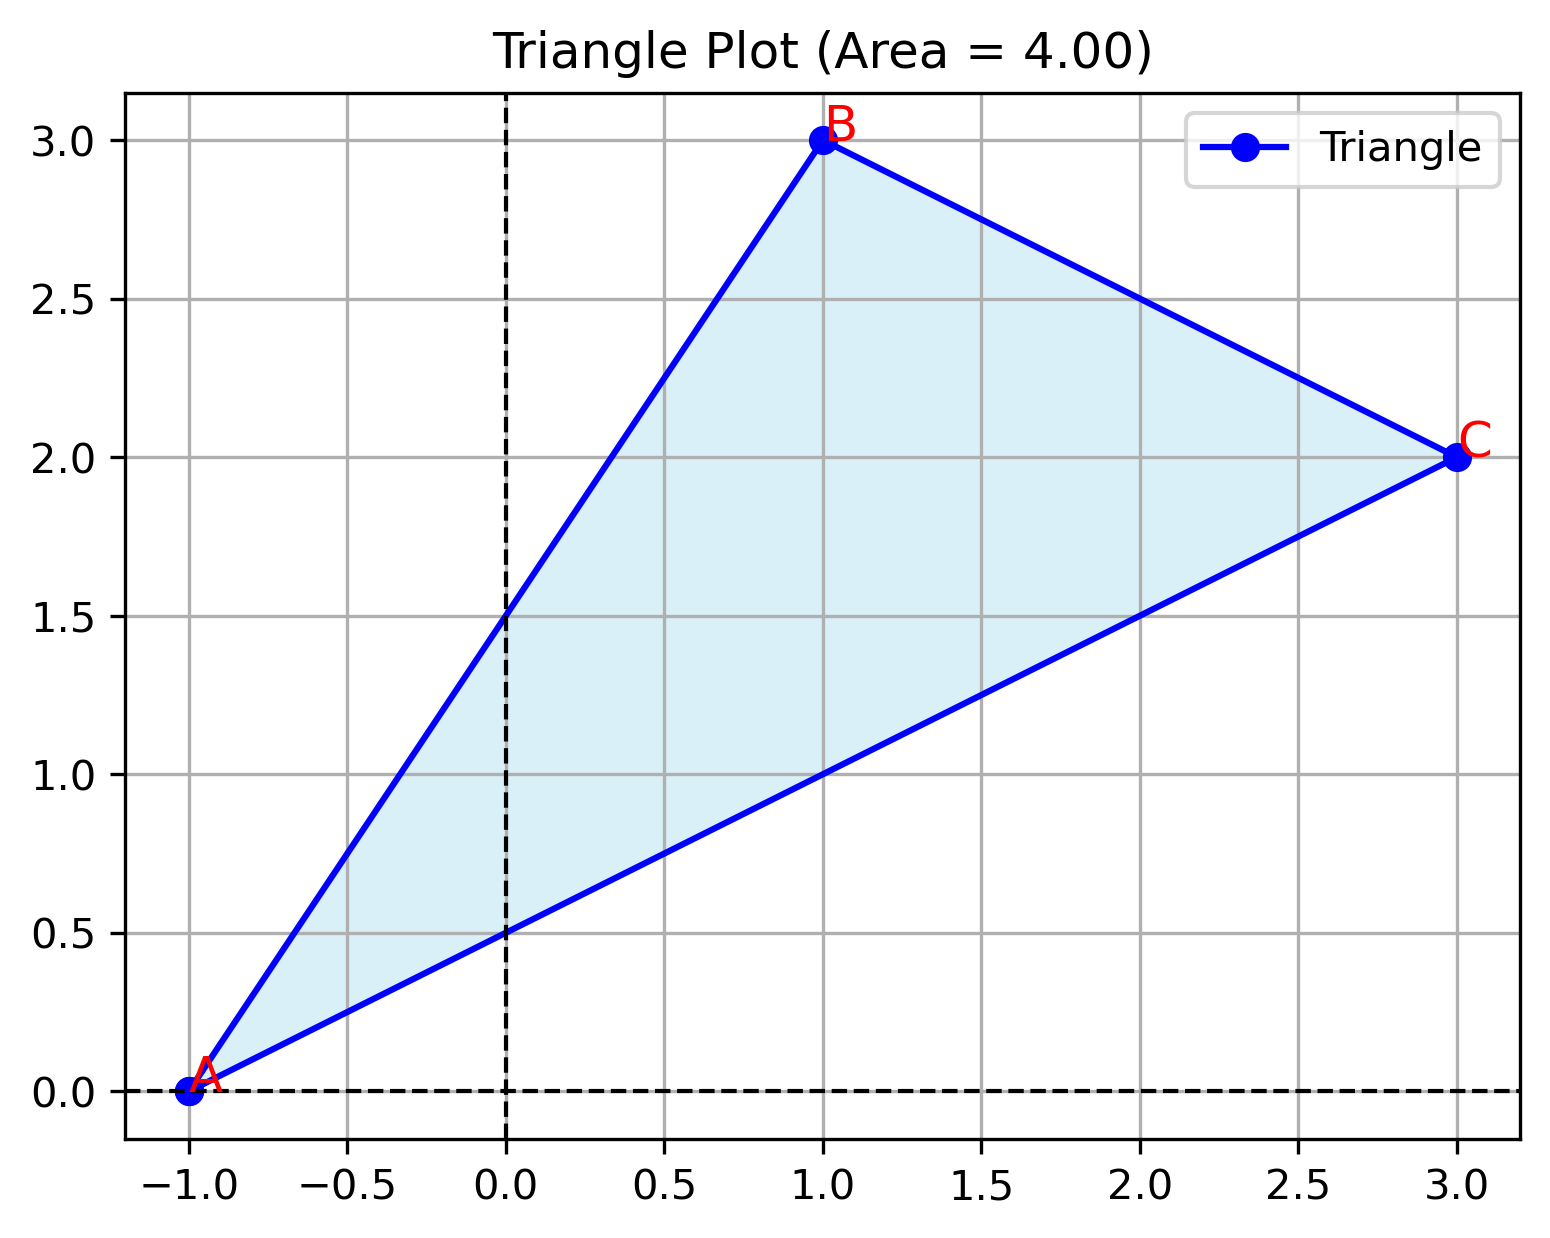
\includegraphics[width=0.7\linewidth]{../figs/triangle_plot.png}
   \caption{}
  \label{stemplot}
\end{figure}


\end{document}
